%\section{Personal-PCFG, an individual oriented password cracker}
\section{Personal-PCFG}
\label{personalpcfg}
After investigating the correlation between personal information and user passwords 
through measurement and quantification, we further study their potential usage to crack passwords
from an attacker's point of view. Based on PCFG
approach~\cite{weir2009password},  we develop Personal-PCFG as an individual-oriented
password cracker that can generate personalized guesses towards a targeted user by exploiting the already known personal information.


\subsection{Attack Scenarios}
We assume that the attacker knows certain amount of personal information
about the targets. The attacker can be an evil neighbor, a curious
friend, a jealous husband, a blackmailer, or even a company that buys
personal information from other companies. Under these conditions,
targeted personal information is rather easy to obtain by knowing the
victim personally or searching online, especially on social networks
sites (SNS)~\cite{gross2005information, krishnamurthy2009leakage}.
Personal-PCFG can be used in both offline and online attacks. 

In traditional offline password attacks, attackers usually steal
hashed passwords from victim systems, and then try to find out the
unhashed values of these passwords. As a secure hash function cannot
be simply reversed, the most popular attacking strategy is to guess
and verify passwords by brute force. Each guess is verified by hashing
a password (salt needs to be added) from a password dictionary and
comparing the result to the hashed values in the leaked password
database. High-probability password guesses can usually match many
hashed values in the password database and thus are expected to be
tried first. For offline attacks, Personal-PCFG is much faster in
guessing out the correct password than conventional methods since it
can generate high-probability personalized passwords and verify them
first.

For online attack, since the attacker does not even have a hashed
password database, he or she instead tries to directly log in the real
systems by guessing the passwords. It is more difficult to succeed in
online attacks than offline attacks because online service systems
usually have restrictions on login attempts for a given period of
time. If the attempt quota has been reached without inputting a
correct password, the account may be locked for some time or even
permanently unless certain actions are taken (e.g., call the service
provider). Therefore, online attacks require very accurate guesses, which can be achieved by
integrating personal information. Personal-PCFG is able to crack
around 1 out of 20 passwords within only 5 guesses.

\subsection{A Revisit of PCFG}
Personal-PCFG is based on the basic idea of PCFG
method~\cite{weir2009password} and provide an extension to further
improve its efficiency. Before we introduce Personal-PCFG, we briefly
revisit principles of PCFG. PCFG pre-processes
passwords and generates base password structures such as $"L_5D_3S_1"$ for each
of the passwords. Starting from high-probability structures, PCFG
method substitutes the ``D'' and ``S'' segments using segments of same
length learned from the training set. These substitute segments are
ranked by probability of occurring learned from the training set. Therefore high
probability segments will be tried first. One base structure may have
a number of substitutions, for example, $"L_5D_3S_1"$ can have
$"L_5123!"$ and $"L_5691!"$ as its substitutions. These new
representations are called pre-terminal structures. No ``L'' segment
is currently substituted since the space of alpha strings is too large
to learn from the training set. Next, these pre-terminals are ranked
from high probability to low probability. Finally ``L'' segments
are substituted using a dictionary to generate actual guesses. 
Besides the basic idea, PCFG
method also carries an efficient algorithm to enumerate passwords from
high probability to low probability on the fly. These
guesses are hashed to compare with the values in password
databases. Since PCFG can generate statistically high probability
password first, it can significantly reduce the guessing number of
traditional dictionary attacks.

\subsection{Personal-PCFG}
Personal-PCFG leverages the basic idea of PCFG. Besides ``L'',
``D'', and ``S'' symbols in PCFG, we add more semantic symbols
including ``B'' for birthday, ``N'' for name, ``E'' for email address,
``A'' for account name, ``C'' for cellphone number, and ``I'' for ID
number. Richer semantics makes Personal-PCFG more accurate in guessing
passwords. To make Personal-PCFG work, an additional personal information matching phase
and an adaptive-substitution phase are added to the original PCFG
method. Therefore, Personal-PCFG has 4 phases and the output of each phase will be fed to the next phase as input. The output of last phase is the actual guesses for trying. We now describe each phase in detail along with simple examples. 

%the goal of each phase; any connection between phases? how many
%phases in total?
 

\subsubsection{Personal Information Matching}
Given a password string, we first match the entire password or a
substring of the password to its personal information. The detailed
algorithm is similar to Algorithm~\ref{alg1}. However, this time we
also record the length of the matching segment. We replace the matched
segments in password with corresponding symbols and mark the symbols
with length. Unmatched segments remain unchanged. For instance, we
assume Alice was born in August 16, 1988 and her password is
``helloalice816!''. The matching phase will replace ``alice'' with
``$N_5$" and ``816'' with ``$B_3$". The leftover ``hello'' is kept
unchanged. Therefore the outcome of this phase is ``$helloN_5B_3!$".

\subsubsection{Password Pre-processing}
This phase is similar to the pre-processing routine of the original
PCFG; however, based on the output of personal information matching
phase, the segments already matched to personal information will not
be processed. For instance, the sample structure
``$helloN_5B_3!$" will be updated to ``$L_5N_5B_3S_1$" in this phase.  Now the
password is fully described by semantic symbols of Personal-PCFG, 
and the output in this phase provides base structures for
Personal-PCFG.

\subsubsection{Guess Generation}
Similar to the original PCFG, we replace ``D'' and ``S''
symbols with actual strings learned from the training set in
descending probability order. ``L'' symbols are replaced with words
from a dictionary. Similar to PCFG~\cite{weir2009password}, we output
the results on the fly so we do not need to wait all possibilities for
guesses are calculated and sorted. The results are kept outputting for
next step. Note that we have not replaced any symbols for personal
information so the guesses are still not actual guesses. We do not
handle personal information in this step, since personal information
for each user is likely to be different and personal information
symbols can only be substituted until the target is specific. 
%
Therefore, in this phase our base structures only generate
pre-terminals, which are partial guesses that contain part of actual
guesses and part of Personal-PCFG semantic symbols. For instance, the
example ``$L_5N_5B_3S_1$" is instantiated to ``$helloN_5B_3!$" if
``hello'' is the first 5-symbol long string in the input dictionary
and ``!'' has highest probability of occurring among 1 symbol special
character in the training set. Note that for ``L'' segments, each word
of the same length has the same probability. The probability of
``hello'' is simply $1\over N$, in which $N$ is the total number of
words of length 5 in the input dictionary.

\subsubsection{Adaptive Substitution}
In the original PCFG, the output of guess generation can be
applied to any target user. However, in Personal-PCFG, the guesses
will be further instantiated with personal information, which are
specific to only one target user.  Each personal information symbol is
replaced by corresponding personal information of the same length. If
there are multiple candidates of the same length, all of them will be
included for trial. In our example $helloN_5B_3!$, $N_5$ will be
directly replaced by ``alice''. However, since $B_3$ has many
candidate segments and any length 3 substring of ``19880816'' may be a
candidate, the guesses include all substrings such as
``helloalice198!'', ``helloalice988!'', $\ldots$,
``helloalice816!''. We then try these candidate guesses one by one
until we find out that the last candidate matches exactly the password
of Alice. Note that on the opposite of having multiple candidate, not
all personal information segments can be replaced since the same
length segments may not always be available. For instance, a
pre-terminal structure $helloN_6B_3!$ is not suitable for Alice since
her name is at most 5 symbols long. In this case no guesses from this
structure should be generated for Alice.

\begin{figure}[t]
  \centering
  \caption{ Compare PCFG and Personal-PCFG.}{}
  \label{f3}
  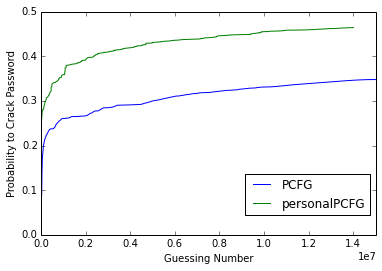
\includegraphics[width=0.4\textwidth]{fig/cmp}
\vspace{-0.1in}
\end{figure}

\subsection{Cracking Results}
We compare the performance of Personal-PCFG and the
original PCFG using the 12306 dataset, which has 131,389 users.  We 
use half of the dataset as the training set,
and the other half as the testing set.  For the ``L" segments, both
methods need to use a dictionary, which is a critical part for password
cracking. To eliminate the effect of unfair dictionary selection, we
use ``perfect'' dictionaries in both methods. Perfect dictionaries are
dictionaries we collected directly from the testing set, so that any
string in the dictionary is useful and any letter segments in the passwords
must appear in the dictionary. Thus, a perfect dictionary is a
guarantee to find correct alpha strings efficiently. In our study, both PCFG perfect dictionary and Personal-PCFG perfect dictionary contain 15,000 to 17,000 entries.

Most previous works on password cracking use {\em guessing number} as
a metric to compare their performance; however, we propose to use {\em
  hashing number} to evaluate Personal-PCFG. 
%
Because hashing operations are the bottleneck of password cracking
attacks, it is more reasonable to compare hashing number instead of
guessing number. Researchers use guessing number in their works
because the guessing number is independent of password dataset size
and one hashed guess can be compared to all the passwords in the
dataset. However, because almost all modern password datasets are
protected by the salt mechanism, each non-personalized guess still
needs to be padded by the individual salt value for each account
before hashing. Therefore, a dataset of $N$ passwords requires $N$
hashes to verify one guess. In Personal-PCFG, one guess is usually
personalized to test on one specific password so that it requires only $1$
hash to verify a guess. 

\begin{figure}[t]
  \centering
  \caption{PCFG and Personal-PCFG -- Online attacks.}{}
  \label{cmp100}
  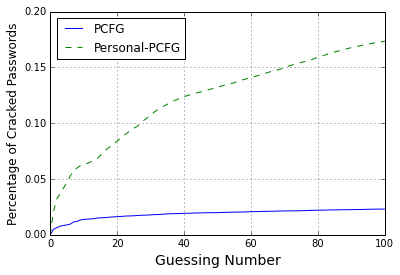
\includegraphics[width=0.4\textwidth]{fig/cmp100}
\vspace{-0.1in}
\end{figure}
Figure~\ref{f3} shows the comparison of the original PCFG and
Personal-PCFG using average hashing number. We compute the probability
of a password to be cracked given various hashing
numbers. Figure~\ref{f3} implies that generally Personal-PCFG works
substantially better than original PCFG. With a moderate size of 500,000 hashes
Personal-PCFG achieves a similar success rate that can be achieved with
over 200 million hashes by original PCFG. That is to
say, Personal-PCFG can crack password much faster than PCFG
does.  Moreover, Personal-PCFG is able to cover a larger password space
than PCFG. This is because personal information provides rich
personalized strings that may not appear in the dictionaries or training set.
%
It is not surprising that both PCFG and Personal-PCFG can crack
passwords quickly when they just start, since both methods always try
high probability guesses first. However, the lines become relatively
flat when the guessing number is growing large.

 \begin{figure}[t]
  \centering
  \caption{Representative Points -- Online attacks.}{}
  \label{points}
  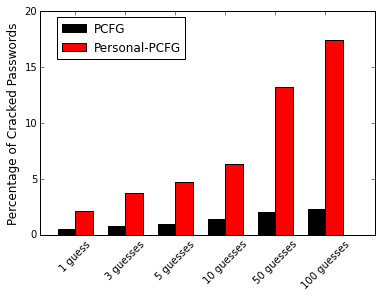
\includegraphics[width=0.4\textwidth]{fig/online}
\vspace{-0.15in}
\end{figure}
%online attacks

Personal-PCFG not only improve the cracking efficiency in offline
attacks, but also increase the guessing success opportunity in online
attacks. Online attacks are only able to try a small number of guesses
in a certain time period due to the system constrains on the login
attempts. Therefore we limit the guesses to be at most 100 times. We present the results in Figure~\ref{cmp100}, from which it can seen that
Personal-PCFG is able to crack 309\% to 634\% more passwords than
original PCFG. We then show several representative guessing numbers in Figure~\ref{points}. For a typical system that allows 5
attempts to input the correct passwords, Personal-PCFG is able to
crack 4.8\% passwords within only 5 guesses. Meanwhile the percentage
is just 0.9\% for original PCFG, and it takes around 2000 more guesses
for PCFG to reach a success rate of 4.8\%. Thus, Personal-PCFG is more
efficient to crack the correct passwords within only a small number of
guesses.

We conclude that Personal-PCFG substantially outperforms PCFG in both online and
offline attacks due to the integration of the personal
information into password guessing. On the other hand, the extra
requirement of Personal-PCFG on personal information can be satisfied
by knowing the victim personally or searching on social networks sites
(SNS).

